\documentclass{beamer}

\usepackage[utf8]{inputenc}
\usepackage[spanish,es-noshorthands]{babel}
\usepackage[utf8]{inputenc}
\usepackage{amssymb,amsthm,amsmath,tikz,graphicx,caption,subcaption}
\graphicspath{ {./images/} }
\usetikzlibrary{intersections, arrows.meta, automata, er, calc, backgrounds, mindmap, folding, patterns, decorations.markings, fit,shadings, matrix, positioning, arrows, through}
\usetheme{PaloAlto}
\usecolortheme{seahorse}

\definecolor{color1}{RGB}{38,70,83}
\definecolor{color2}{RGB}{42,157,143}
\definecolor{color3}{RGB}{233,196,106}
\definecolor{color4}{RGB}{244,162,97}
\definecolor{color5}{RGB}{231,111,81}

\title{Algoritmos de compresión en medios de preservación y difusión cultural}
\author{Juan de la Cruz García García}
\institute{Actualización Científica - Master en Matemáticas - Universidad de Cádiz}
\date{2021.03.14}

\begin{document}

\frame{\titlepage}

\begin{frame}
\frametitle{Contenido}
\tableofcontents
\end{frame}

\section{Introducción}

\begin{frame}
\frametitle{¿De qué hablaremos hoy?}

\begin{tikzpicture}
	[
	node distance=0.5cm and 1cm,
        destacado/.style={
            rectangle, 
            rounded corners,
            draw=color1!40!white,
            very thick,
            fill=color2!40!white,
            align=center,
            text width=2.5cm
        }, 
        explicacion/.style={
	    rectangle, 
	    rounded corners,
            align=left,
            draw=color4!40!white,
            fill=color3!40!white,
            very thick,
            text width=6.25cm
        }, 
        flechaAccion/.style={
            ->,
            thick
        }
    ]
    \node(algoritmos) [destacado] {Algoritmos de compresión};
    \node(medios) [destacado, below=of algoritmos] {Medios};
    \node(preservar) [destacado, below=0.75cm of medios] {Preservar};
    \node(difundir) [destacado, below=1.25cm of preservar] {Difusión};
    \node(cultura) [destacado, below=1cm of difundir] {Cultura};

    \node(explicacionAlgoritmos) [explicacion, right=of algoritmos] {Matemáticas};
    \node(explicacionMedios) [explicacion, right=of medios] {Formatos, objetos, vías};
    \node(explicacionPreservar) [explicacion, right=of preservar] {Proteger, resguardar anticipadamente a alguien o algo, de algún daño o peligro};
    \node(explicacionDifundir) [explicacion, right=of difundir] {Propagar o divulgar conocimientos, noticias, actitudes, costumbres, modas, etc};
    \node(explicacionCultura) [explicacion, right=of cultura] {Música, Literatura, Cine, Pintura, Escultura...};

    \draw[flechaAccion] (algoritmos)--(explicacionAlgoritmos);
    \draw[flechaAccion] (medios)--(explicacionMedios);
    \draw[flechaAccion] (preservar)--(explicacionPreservar);
    \draw[flechaAccion] (difundir)--(explicacionDifundir);
    \draw[flechaAccion] (cultura)--(explicacionCultura);
\end{tikzpicture}
\end{frame}

\section{Algoritmos de compresión}
\begin{frame}
    \frametitle{Algoritmos de compresión}
    \centering
		\setbeamercovered{dynamic}
		\begin{tikzpicture}[scale=0.75,transform shape]
		\path[mindmap,concept color=color1!40!white,text=black]
		node[concept] {Algoritmos de compresión}
		[clockwise from=-45]
		    child[concept color=color2!40!white] {
			node[concept] {Con pérdida}
			[clockwise from=45]
			child { node[concept] {Transforma\-da de Coseno Discreta (DCT)} }
			child { node[concept] {MCDT} }
			}  
			child[concept color=color3!40!white]{
			node[concept] {Sin pérdida}
			[clockwise from=-10]
			child {node[concept]{LZ77}}
			child {node[concept]{LZR}}
			child {node[concept]{LZSS}}
			child {node[concept]{LZMA}}
            child {node[concept]{bzip2}}
		};
		
		\end{tikzpicture}
\end{frame}

\begin{frame}
    \frametitle{Algoritmos, Formatos y Estándares}
    \centering
		\setbeamercovered{dynamic}
		\begin{tikzpicture}
            \draw[black,thick,fill=color1!40!white] (0,0) circle (3.5cm);
            \node[] at (0,3){Estandar};
            \draw[black,thick,fill=color2!40!white] (0,0) circle (2.5cm);
            \node[] at (0,2){Formato};
            \draw[black,thick,fill=color3!40!white] (0,0) circle (1.5cm);
            \node[] at (0,0){Algoritmo};
		\end{tikzpicture}
\end{frame}

\begin{frame}
    \frametitle{Nomenclatura casual}
    \centering
		\setbeamercovered{dynamic}
		\begin{tikzpicture}[scale=0.75,transform shape]
		\path[mindmap,concept color=color1!40!white,text=black]
		node[concept] {Formatos de compresión}
		[clockwise from=-45]
		    child[concept color=color2!40!white] {
			node[concept] {Con pérdida}
			[clockwise from=90]
			child { node[concept] {JPG} }
			child { node[concept] {WebP} }
            child { node[concept] {MP3} }
            child { node[concept] {H.264} }
			}  
			child[concept color=color3!40!white]{
			node[concept] {Sin pérdida}
			[clockwise from=-10]
			child {node[concept]{PNG}}
			child {node[concept]{BMP}}
			child {node[concept]{AVI}}
			child {node[concept]{ALAC}}
            child {node[concept]{WAV}}
		};
		
		\end{tikzpicture}
\end{frame}
\section{Formatos Analógicos y digitales}
\begin{frame}
    \frametitle{Medios}
    \centering
		\setbeamercovered{dynamic}
		\begin{tikzpicture}[scale=0.75,transform shape]
		\path[mindmap,concept color=color1!40!white,text=black]
		node[concept] {Medios de almacenaje}
		[clockwise from=-45]
		    child[concept color=color2!40!white] {node[concept] {Físicos} }
			child[concept color=color3!40!white]{ node[concept] {Digitales} }
		;
		
		\end{tikzpicture}
\end{frame}

\begin{frame}
    \frametitle{Ejemplos de medios físicos}
    \centering
    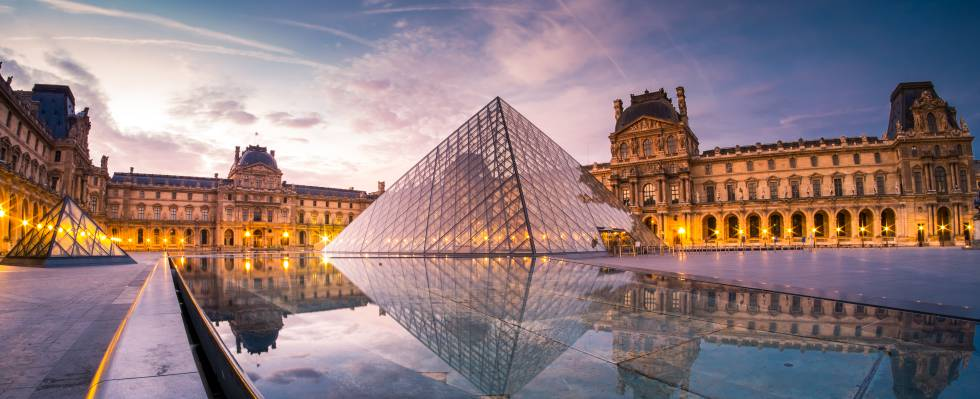
\includegraphics[scale=0.25]{louvre}    

    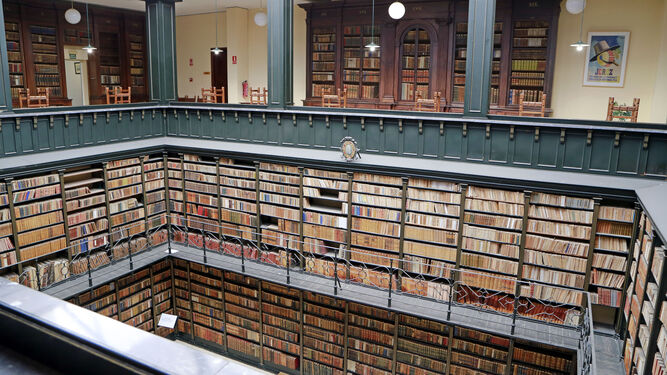
\includegraphics[scale=0.75]{biblioteca} 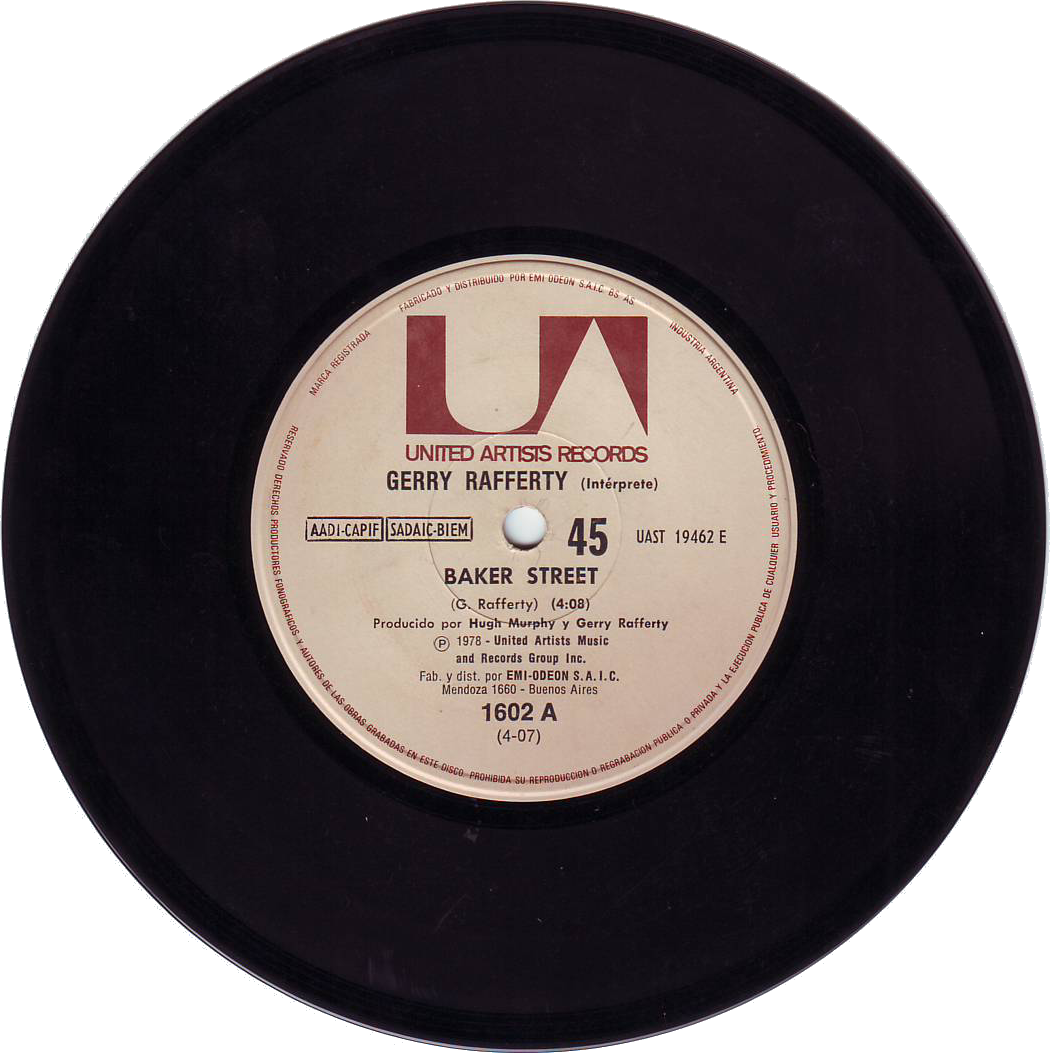
\includegraphics[scale=0.2]{vinilo}    
\end{frame}

\begin{frame}
    \frametitle{Medios Físicos}
    \centering
    \begin{exampleblock}{Ventajas}
        \begin{enumerate}
            \item La obra original da valor.
            \item La copia es muy compleja de hacer.
            \item Favorece la industria alrededor de la obra.
        \end{enumerate}
    \end{exampleblock}
    \begin{block}{Desventajas}
        \begin{enumerate}
            \item No siempre puede contarse con los originales.
            \item Expone a la obra original a peligros.
            \item La industria no está preparada para el cambio de paradigma.
        \end{enumerate}
    \end{block}
\end{frame}

\begin{frame}
    \frametitle{Ejemplos de medios digitales}
    \centering
    
\includegraphics[scale=0.05]{cd}
    
\includegraphics[scale=0.2]{spotify}

    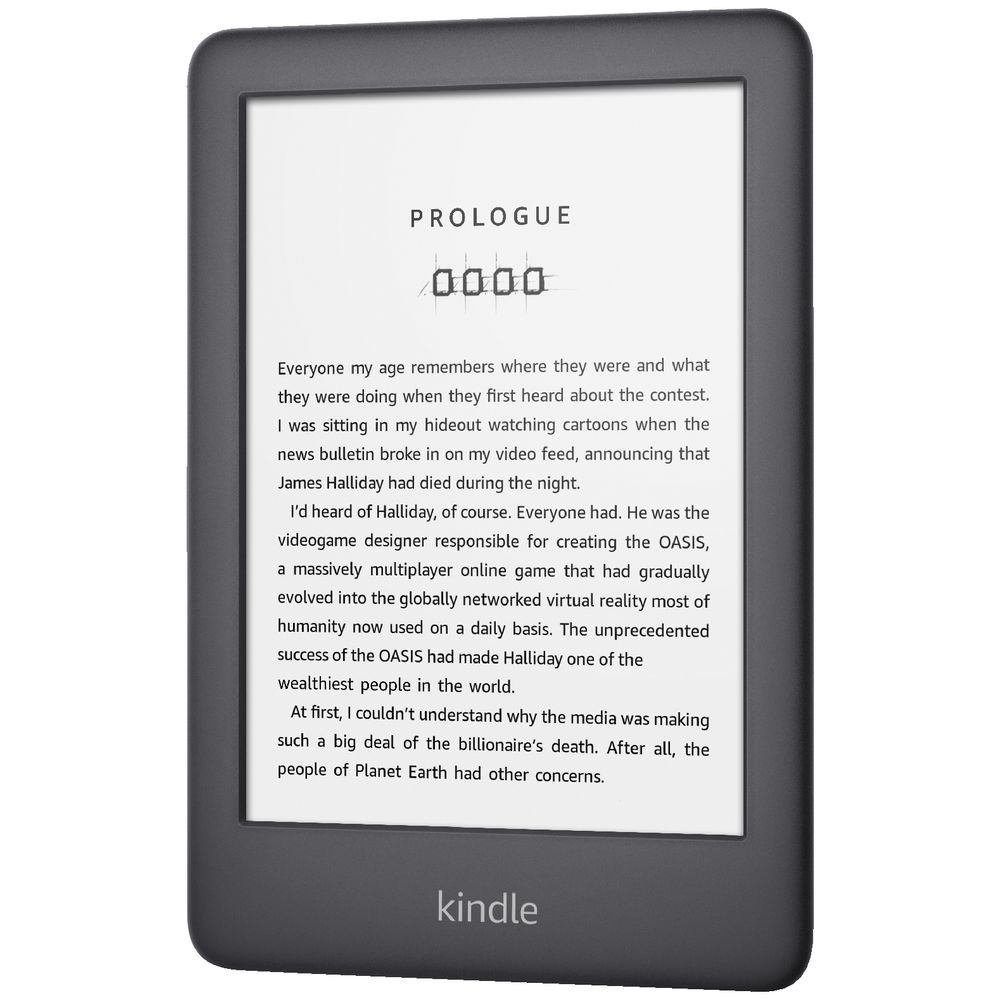
\includegraphics[scale=0.1]{kindle}
    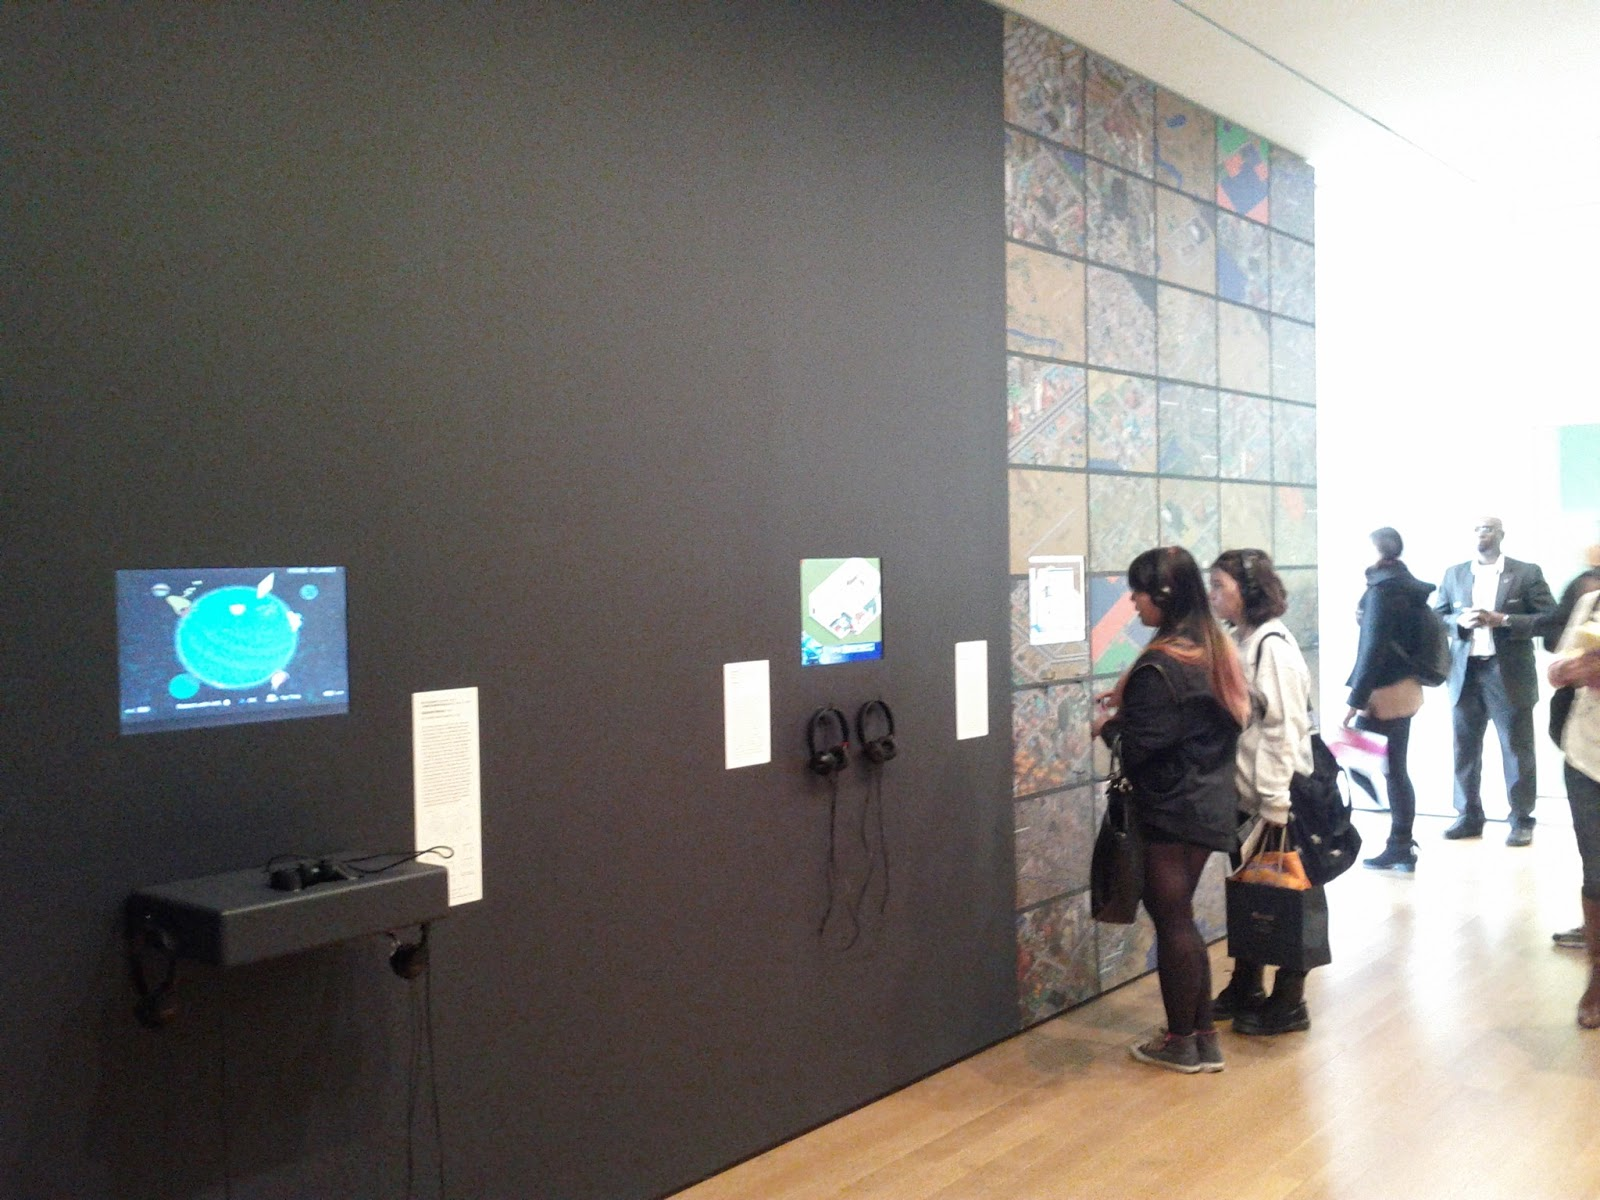
\includegraphics[scale=0.1]{moma}
   
\end{frame}

\begin{frame}
    \frametitle{Medios Digitales}
    \centering
    \begin{exampleblock}{Ventajas}
        \begin{enumerate}
            \item Democratiza el acceso a las obras culturales.
            \item Salvaguarda el original de deterioro y/o destrucción.
            \item Crea otra industria alrededor de la obra.
        \end{enumerate}
    \end{exampleblock}
    \begin{block}{Desventajas}
        \begin{enumerate}
            \item El original pierde valor, si es que existe.
            \item La réplica sin permiso es muy fácil de hacer.
            \item Se pierden matices si la preservación es errónea.
        \end{enumerate}
    \end{block}
\end{frame}

\begin{frame}
    \frametitle{Factores para la preservación y difusión}
    
    \begin{tikzpicture}
        [
        node distance=0.5cm and 2cm,
            destacado/.style={
                circle, 
                draw=color1!40!white,
                very thick,
                fill=color2!40!white,
                align=center,
                text width=2.5cm
            }, 
            consecuencia/.style={
                rectangle, 
                rounded corners,
                draw=color3!40!white,
                very thick,
                fill=color4!40!white,
                align=center,
                text width=2.5cm
            },
            flechaAccion/.style={
                ->,
                thick
            }
        ]
        \node(ficheros) [destacado] {Ficheros};
        \node(espacio) [consecuencia, text=red, right=of ficheros] {Tamaño};
        \node(seguridad) [consecuencia, above=of espacio] {Seguridad};
        \node(accesibilidad) [consecuencia, above=of seguridad] {Accesibilidad};
        \node(fidelidad) [consecuencia, text=red, below=of espacio] {Fidelidad};
        \node(disponibilidad) [consecuencia, below=of fidelidad] {Disponibilidad};

        \draw[flechaAccion] (ficheros)--(espacio.west);
        \draw[flechaAccion] (ficheros)--(seguridad.west);
        \draw[flechaAccion] (ficheros)--(accesibilidad.west);
        \draw[flechaAccion] (ficheros)--(fidelidad.west);
        \draw[flechaAccion] (ficheros)--(disponibilidad.west);
    \end{tikzpicture}
\end{frame}

\begin{frame}
    \frametitle{Correlación entre el Tamaño y la Fidelidad}
    \centering
    \begin{tikzpicture}[scale=2.5, line cap=round]
        \draw [step=0.1, very thin, lightgray] (0, 0) grid (3,2);
        \draw (0, 0) -- (3, 0);
        \draw (0, 0) -- (0, 2);
        \node[label={[rotate=90]right:Fidelidad}] at (-0.2,0) {};
        \node[label={right:Tamaño}] at (0,-0.2) {};
        \draw [red, very thick](0,0) to [out=0, in=180] (3,2);
    \end{tikzpicture}
\end{frame}

\section{Algoritmos de compresión con pérdidas}
\begin{frame}
    \frametitle{Compresión con pérdidas}
   \centering
    \begin{exampleblock}{Ventajas}
        \begin{enumerate}
            \item Se tiene un fichero muy parecido al original
            \item El fichero es pequeño, por lo que es fácil archivarlo y distribuirlo.
        \end{enumerate}
    \end{exampleblock}
    \begin{block}{Desventajas}
        \begin{enumerate}
            \item El fichero jamás será idéntico al original.
            \item La compresión requiere tiempo de procesado.
            \item Si la compresión es muy agresiva, la obra expuesta puede ser irremediablemente deteriorada.
        \end{enumerate}
    \end{block}
\end{frame}

\begin{frame}
    \frametitle{Ejemplo: Fichero de sonido}
    \centering
    \begin{tikzpicture}[scale=2.5, line cap=round]
        %\draw [step=0.1, very thin, lightgray] (0, -1) grid (3,1);
        \draw (0, 0) -- (3, 0);
        \draw (0, -1) -- (0, 1);
        \draw [color1](0,-0.5) -- (0.1, 0.185982925) --
        (0.2, -0.119775969) --
        (0.3, 0.5) --
        (0.4, -0.57466858) --
        (0.5, 0.5843802) --
        (0.6, -0.2) --
        (0.7, 0.438) --
        (0.8, -0.511154235) --
        (0.9, 0.615703089) --
        (1, -0.38632) --
        (1.1, 0.851216038) --
        (1.2, -0.39368972) --
        (1.3, 0.966531713) --
        (1.4, -0.797318728) --
        (1.5, 0.31682) --
        (1.6, -0.555847506) --
        (1.7, 0.584478575) --
        (1.8, -0.832338247) --
        (1.9, 0.545636247) --
        (2, -0.98283762873) --
        (2.1, 0.32868) --
        (2.2, -0.82736827) --
        (2.3, 0.293897) --
        (2.4, -0.777391848) --
        (2.5, 0.779169846) --
        (2.6, -0.2397823) --
        (2.7, 0.500918175) --
        (2.8, -0.651726055) --
        (2.9, 0.626304584) --
        (3, -0.2934729);
    \end{tikzpicture}
\end{frame}

\begin{frame}
    \frametitle{Ejemplo: Fichero de sonido}
    \centering
    \begin{tikzpicture}[scale=2.5, line cap=round]
        %\draw [step=0.1, very thin, lightgray] (0, -1) grid (3,1);
        \draw (0, 0) -- (3, 0);
        \draw (0, -1) -- (0, 1);
        \filldraw [color2!20!white] (0, 0.4) rectangle (3,1); 
        \filldraw [color2!20!white] (0, -0.4) rectangle (3,-1); 
        \draw [color1](0,-0.5) -- (0.1, 0.185982925) --
        (0.2, -0.119775969) --
        (0.3, 0.5) --
        (0.4, -0.57466858) --
        (0.5, 0.5843802) --
        (0.6, -0.2) --
        (0.7, 0.438) --
        (0.8, -0.511154235) --
        (0.9, 0.615703089) --
        (1, -0.38632) --
        (1.1, 0.851216038) --
        (1.2, -0.39368972) --
        (1.3, 0.966531713) --
        (1.4, -0.797318728) --
        (1.5, 0.31682) --
        (1.6, -0.555847506) --
        (1.7, 0.584478575) --
        (1.8, -0.832338247) --
        (1.9, 0.545636247) --
        (2, -0.98283762873) --
        (2.1, 0.32868) --
        (2.2, -0.82736827) --
        (2.3, 0.293897) --
        (2.4, -0.777391848) --
        (2.5, 0.779169846) --
        (2.6, -0.2397823) --
        (2.7, 0.500918175) --
        (2.8, -0.651726055) --
        (2.9, 0.626304584) --
        (3, -0.2934729);
    \end{tikzpicture}

    Parte del espectro auditivo no lo percibe el oído humano...
\end{frame}

\begin{frame}
    \frametitle{Ejemplo: Fichero de sonido}
    \centering
    \begin{tikzpicture}[scale=2.5, line cap=round]
        %\draw [step=0.1, very thin, lightgray] (0, -1) grid (3,1);
        \draw (0, 0) -- (3, 0);
        \draw (0, -1) -- (0, 1);
        
        \draw [color1](0,-0.5) -- (0.1, 0.185982925) --
        (0.2, -0.119775969) --
        (0.3, 0.5) --
        (0.4, -0.57466858) --
        (0.5, 0.5843802) --
        (0.6, -0.2) --
        (0.7, 0.438) --
        (0.8, -0.511154235) --
        (0.9, 0.615703089) --
        (1, -0.38632) --
        (1.1, 0.851216038) --
        (1.2, -0.39368972) --
        (1.3, 0.966531713) --
        (1.4, -0.797318728) --
        (1.5, 0.31682) --
        (1.6, -0.555847506) --
        (1.7, 0.584478575) --
        (1.8, -0.832338247) --
        (1.9, 0.545636247) --
        (2, -0.98283762873) --
        (2.1, 0.32868) --
        (2.2, -0.82736827) --
        (2.3, 0.293897) --
        (2.4, -0.777391848) --
        (2.5, 0.779169846) --
        (2.6, -0.2397823) --
        (2.7, 0.500918175) --
        (2.8, -0.651726055) --
        (2.9, 0.626304584) --
        (3, -0.2934729);
        \filldraw [white] (0.01, 0.4) rectangle (3,1); 
        \filldraw [white] (0.01, -0.4) rectangle (3,-1); 
    \end{tikzpicture}

    ...Se puede quitar y nos ahorramos unos MB!
\end{frame}

\begin{frame}
    \frametitle{Ejemplo: Fichero de imagen}
    \centering
    \begin{tikzpicture}[scale=2.5, line cap=round]
        \draw[step=1cm] (1,1) grid (4,4);
        \filldraw [color1] (1, 1) rectangle (2,2); 
        \filldraw [color2] (1, 2) rectangle (2,3); 
        \filldraw [color3] (1, 3) rectangle (2,4);
        
        \filldraw [color4] (2, 1) rectangle (3,2); 
        \filldraw [color5] (2, 2) rectangle (3,3); 
        \filldraw [color1] (2, 3) rectangle (3,4);

        \filldraw [color3] (3, 1) rectangle (4,2); 
        \filldraw [color2] (3, 2) rectangle (4,3); 
        \filldraw [color5] (3, 3) rectangle (4,4);
    \end{tikzpicture}
\end{frame}

\begin{frame}
    \frametitle{Ejemplo: Fichero de imagen}
    \centering
    \begin{tikzpicture}[scale=2.5, line cap=round]
        \draw[step=1cm] (1,1) grid (4,4);
        \filldraw [color1] (1, 1) rectangle (2,2); 
        \filldraw [color1] (1, 2) rectangle (2,3); 
        \filldraw [color3] (1, 3) rectangle (2,4);
        
        \filldraw [color3] (2, 1) rectangle (3,2); 
        \filldraw [color3] (2, 2) rectangle (3,3); 
        \filldraw [color1] (2, 3) rectangle (3,4);

        \filldraw [color3] (3, 1) rectangle (4,2); 
        \filldraw [color1] (3, 2) rectangle (4,3); 
        \filldraw [color3] (3, 3) rectangle (4,4);
    \end{tikzpicture}
\end{frame}

\begin{frame}
    \frametitle{Ejemplo: Fichero de imagen}
    \centering
    
\includegraphics[scale=0.8]{uca_HR} 
    
\includegraphics[scale=0.8]{uca_LR}


    \includegraphics[scale=0.5]{tamaño_HR}
    \includegraphics[scale=0.5]{tamaño_LR}
\end{frame}

\section{Algoritmos de compresión sin pérdidas}
\begin{frame}
    \frametitle{Compresión sin pérdidas}
    \centering
    \begin{exampleblock}{Ventajas}
        \begin{enumerate}
            \item Se tiene un fichero idéntico al original, con todos los matices.
            \item En un cambio de tecnología, es posible utilizarlo como fuente.
        \end{enumerate}
    \end{exampleblock}
    \begin{block}{Desventajas}
        \begin{enumerate}
            \item El fichero puede ser de gran tamaño.
            \item Su disponibilidad y accesibilidad se comprometen.
            \item El tiempo de procesado es aún mayor.
            \item Para la mayoría de los casos puede ser innecesario.
        \end{enumerate}
    \end{block}
\end{frame}

\begin{frame}
    \frametitle{Ejemplo: Run-length Encoding}
    \begin{columns}
        \column{0.5\textwidth}
            \begin{tikzpicture}[line cap=round]
                \filldraw [color1] (1, 7) rectangle (2,8); \filldraw [color1] (2, 7) rectangle (3,8); \filldraw [color1] (3, 7) rectangle (4,8); 
                \filldraw [color1] (1, 6) rectangle (2,7); \filldraw [color2] (2, 6) rectangle (3,7); \filldraw [color2] (3, 6) rectangle (4,7); 
                \filldraw [color2] (1, 5) rectangle (2,6); \filldraw [color2] (2, 5) rectangle (3,6); \filldraw [color2] (3, 5) rectangle (4,6); 
                \filldraw [color2] (1, 4) rectangle (2,5); \filldraw [color3] (2, 4) rectangle (3,5); \filldraw [color3] (3, 4) rectangle (4,5); 
                \filldraw [color3] (1, 3) rectangle (2,4); \filldraw [color1] (2, 3) rectangle (3,4); \filldraw [color1] (3, 3) rectangle (4,4); 
                \filldraw [color1] (1, 2) rectangle (2,3); \filldraw [color1] (2, 2) rectangle (3,3); \filldraw [color2] (3, 2) rectangle (4,3); 
                \filldraw [color2] (1, 1) rectangle (2,2); \filldraw [color2] (2, 1) rectangle (3,2); \filldraw [color2] (3, 1) rectangle (4,2); 

                \draw[step=1cm] (1,1) grid (4,8);
                \node[label={right:3x7x1=21}] at (0.75,0.5) {};
            \end{tikzpicture}
        
        \column{0.5\textwidth}
            \begin{tikzpicture}[line cap=round]
                
                \filldraw [color1] (0, 4) rectangle (2,6); 
                \filldraw [color2] (2, 4) rectangle (4,6); 
                \filldraw [color3] (0, 2) rectangle (2,4); 
                \filldraw [color1] (2, 2) rectangle (4,4); 
                \filldraw [color2] (0, 0) rectangle (2,2); 
                \node[label={[font=\large,text=white]:4}] at (1, 4.5) {};
                \node[label={[font=\large,text=white]:6}] at (3, 4.5) {};
                \node[label={[font=\large,text=white]:3}] at (1, 2.5) {};
                \node[label={[font=\large,text=white]:4}] at (3, 2.5) {};
                \node[label={[font=\large,text=white]:4}] at (1, 0.5) {};

                \draw[step=2cm] (0,0) grid (4,6);
                \node[label={right:RLE: 2x3x2=12}] at (-0.25,-0.75) {};
            \end{tikzpicture}
    \end{columns}
    
\end{frame}

\begin{frame}
    \frametitle{Ejemplo: Diccionario}
    \begin{columns}
        \column{0.5\textwidth}
            \begin{tikzpicture}[line cap=round]
                \filldraw [color1] (1, 7) rectangle (2,8); \filldraw [color1] (2, 7) rectangle (3,8); \filldraw [color1] (3, 7) rectangle (4,8); 
                \filldraw [color1] (1, 6) rectangle (2,7); \filldraw [color2] (2, 6) rectangle (3,7); \filldraw [color2] (3, 6) rectangle (4,7); 
                \filldraw [color2] (1, 5) rectangle (2,6); \filldraw [color2] (2, 5) rectangle (3,6); \filldraw [color2] (3, 5) rectangle (4,6); 
                \filldraw [color2] (1, 4) rectangle (2,5); \filldraw [color3] (2, 4) rectangle (3,5); \filldraw [color3] (3, 4) rectangle (4,5); 
                \filldraw [color3] (1, 3) rectangle (2,4); \filldraw [color1] (2, 3) rectangle (3,4); \filldraw [color1] (3, 3) rectangle (4,4); 
                \filldraw [color1] (1, 2) rectangle (2,3); \filldraw [color1] (2, 2) rectangle (3,3); \filldraw [color2] (3, 2) rectangle (4,3); 
                \filldraw [color2] (1, 1) rectangle (2,2); \filldraw [color2] (2, 1) rectangle (3,2); \filldraw [color2] (3, 1) rectangle (4,2); 

                \draw[step=1cm] (1,1) grid (4,8);
                \node[label={right:3x7x1=21}] at (0.75,0.5) {};
            \end{tikzpicture}
        
        \column{0.5\textwidth}
            \begin{tikzpicture}[scale=0.5,line cap=round]
                
                \filldraw [green!50!black] (0, 4) rectangle (2,6); 
                \filldraw [blue] (2, 4) rectangle (4,6); 
                \filldraw [red] (0, 2) rectangle (2,4); 
                \filldraw [green!50!black] (2, 2) rectangle (4,4); 
                \filldraw [orange] (0, 0) rectangle (2,2); 

                \node[label={[font=\large,text=white]:A}] at (1, 4.25) {};
                \node[label={[font=\large,text=white]:B}] at (3, 4.25) {};
                \node[label={[font=\large,text=white]:C}] at (1, 2.25) {};
                \node[label={[font=\large,text=white]:A}] at (3, 2.25) {};
                \node[label={[font=\large,text=white]:D}] at (1, 0.25) {};

                \draw[step=2cm] (0,0) grid (4,6);
                \node[label={right:Dict: 2x3x1=6}] at (-0.25,-0.75) {};
                \node[label={right:+ traducción}] at (-0.25,-1.75) {};
            \end{tikzpicture}
    \end{columns}
    
\end{frame}

\begin{frame}
    \frametitle{Futuro}
    \centering
    \begin{block}{Machine Learning}
        \begin{itemize}
            \item Redes neuronales que reconocen patrones complejos.
            \item Traducciones más eficientes.
            \item Mezcla de técnicas y paradigmas.
            \item Adaptación de la compresión según factores.
            \begin{itemize}
                \item Disponibilidad.
                \item Conectividad.
                \item Localización.
                \item Aprendizaje.
            \end{itemize}
        \end{itemize}
    \end{block}
\end{frame}

\section{Conveniencia para cada uso}
\begin{frame}
    \frametitle{Libros}
    \begin{block}{Algoritmos con pérdida}
        \begin{itemize}
            \item Facsímiles.
            \item Previsualizaciones y muestras.
        \end{itemize}
    \end{block}
    \begin{exampleblock}{Algoritmos sin pérdida}
        \begin{itemize}
            \item Repositorio digital.
            \item Consulta en biblioteca de originales.
            \item Dispositivos portátiles.
        \end{itemize}
    \end{exampleblock}
\end{frame}

\begin{frame}
    \frametitle{Música}
    \begin{block}{Algoritmos con pérdida}
        \begin{itemize}
            \item Dispositivos portátiles.
            \item Tienda virtual.
            \item Servicios de música bajo demanda.
            \item Lugares con recursos tecnológicos limitados.
        \end{itemize}
    \end{block}
    \begin{exampleblock}{Algoritmos sin pérdida}
        \begin{itemize}
            \item Repositorio digital.
            \item Biblioteca municipal, universidad\dots
            \item Escuelas de música y danza.
        \end{itemize}
    \end{exampleblock}
\end{frame}

\begin{frame}
    \frametitle{Pinturas y Esculturas}
    \begin{block}{Algoritmos con pérdida}
        \begin{itemize}
            \item Exposición virtual.
            \item Catálogo de arte.
            \item Tablets y portátiles en áula de enseñanza.
            \item Repositorio de modelos de impresión en 3D.
        \end{itemize}
    \end{block}
    \begin{exampleblock}{Algoritmos sin pérdida}
        \begin{itemize}
            \item Repositorio digital.
            \item Archivo de un museo.
            \item Servidor de un áula de enseñanza.
        \end{itemize}
    \end{exampleblock}
\end{frame}

\end{document}